% patterns.meta Dots + Stars families.
\usetikzlibrary{patterns.meta}

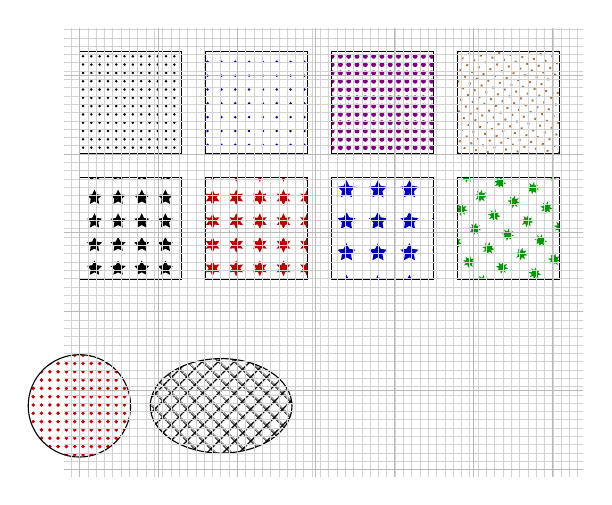
\begin{tikzpicture}[x=1cm,y=1cm]
  % Dots
  \path[draw,pattern={Dots},pattern color=black] (0,0) rectangle +(1.3,1.3);
  \path[draw,pattern={Dots[distance=5pt]},pattern color=blue!70!black] (1.6,0) rectangle +(1.3,1.3);
  \path[draw,pattern={Dots[radius=.9pt]},pattern color=violet] (3.2,0) rectangle +(1.3,1.3);
  \path[draw,pattern={Dots[angle=35,xshift=1pt,yshift=1pt]},pattern color=brown!90!black] (4.8,0) rectangle +(1.3,1.3);

  % Stars
  \path[draw,pattern={Stars},pattern color=black] (0,-1.6) rectangle +(1.3,1.3);
  \path[draw,pattern={Stars[points=6]},pattern color=red!75!black] (1.6,-1.6) rectangle +(1.3,1.3);
  \path[draw,pattern={Stars[distance=4mm,radius=1.2mm]},pattern color=blue!75!black] (3.2,-1.6) rectangle +(1.3,1.3);
  \path[draw,pattern={Stars[angle=35,xshift=1pt,yshift=1pt,points=8,radius=.8mm]},pattern color=green!60!black] (4.8,-1.6) rectangle +(1.3,1.3);

  % Shape checks
  \path[draw,pattern={Dots[radius=.7pt]},pattern color=red!80!black] (0,-3.2) circle[radius=.65];
  \path[draw,pattern={Hatch[angle=45,distance=4pt,line width=.5pt]},pattern color=black] (1.8,-3.2) ellipse[x radius=.9,y radius=.6];

  % Overlay reference grid for easier phase/offset comparison.
  \draw[step=3pt,gray!35,line width=.1pt] (-0.2,-4.1) grid (6.4,1.6);
  \draw[step=1cm,gray!55,line width=.16pt] (-0.2,-4.1) grid (6.4,1.6);
\end{tikzpicture}
